% Poster for the a Fall 2026 agent-evaluation symposium.
% Size: change the two lengths below if the venue specifies otherwise. 48 x 36 in landscape by default.
\documentclass{article}
\usepackage[paperwidth=48in,paperheight=36in,margin=1.0in]{geometry}
\usepackage{lmodern}\usepackage[T1]{fontenc}\usepackage{anyfontsize}
\usepackage{amsmath,amssymb,booktabs,graphicx,xcolor,tcolorbox,qrcode,array}
\tcbuselibrary{skins}
\definecolor{ink}{HTML}{1B1F2A}\definecolor{teal}{HTML}{1F5F7A}\definecolor{red}{HTML}{B83A2A}\definecolor{pale}{HTML}{F4F6F8}\definecolor{mute}{HTML}{5B6270}
\pagestyle{empty}\setlength{\parindent}{0pt}\setlength{\parskip}{0.6em}
\renewcommand{\normalsize}{\fontsize{30}{37}\selectfont}\normalsize
\newcommand{\blocktitle}[1]{{\fontsize{44}{50}\selectfont\bfseries\color{teal}#1}}
\newcommand{\bignum}[1]{{\fontsize{110}{114}\selectfont\bfseries\color{red}#1}}
\tcbset{poster/.style={enhanced,colback=white,colframe=teal!60!black,boxrule=2pt,arc=10pt,left=18pt,right=18pt,top=14pt,bottom=14pt,fonttitle=\fontsize{44}{50}\selectfont\bfseries,coltitle=white,colbacktitle=teal,toptitle=10pt,bottomtitle=10pt}}
\begin{document}
% ---------------- header
\begin{minipage}[t]{0.78\textwidth}
{\fontsize{84}{92}\selectfont\bfseries\color{ink} Auditing the Winner:\\ An Upper Bound on What Critic Disagreement Adds\\ Beyond the Selector on SWE-Agent Trajectories}\\[14pt]
{\fontsize{40}{46}\selectfont Joseph Morante \quad\textcolor{mute}{Algoverse AI Research \quad\textperiodcentered\quad morantejoseph1@gmail.com}}
\end{minipage}\hfill
\begin{minipage}[t]{0.19\textwidth}\raggedleft
\vspace{0pt}\qrcode[height=4.2in]{https://github.com/morantejr/silentfail-bench}\\[8pt]
{\fontsize{26}{30}\selectfont\color{mute} pre-registration, amendments, code, data\\ github.com/morantejr/silentfail-bench}
\end{minipage}

\vspace{18pt}
% ---------------- three columns
\begin{minipage}[t]{0.315\textwidth}\vspace{0pt}
\begin{tcolorbox}[poster,title=The question]
A coding agent tries a task $n$ times; a scoring model picks the best attempt and commits it. \textbf{Silent failure:} the agent says it is done, the scorer agrees, the project's tests fail.

\begin{center}\bignum{35\% and 45\%}\\[4pt]{\fontsize{33}{39}\selectfont of committed trajectories were silent failures\\ (SWE-bench Verified, 34 rows; Multilingual, 77 rows)}\end{center}

The proposed safeguard: a \textbf{disjoint panel of critics}; escalate when they \textbf{disagree}. Audit signals are almost always evaluated on candidate \emph{pools}. A deployed auditor runs \emph{after} selection. We evaluated it where it would run: on the population the selector actually commits, against the selector's own score, with executed gold.
\end{tcolorbox}

\begin{tcolorbox}[poster,title=Setup (pre-registered throughout)]
\begin{itemize}\setlength{\itemsep}{2pt}
\item \texttt{gpt-5-mini} agent, 40-step limit; best-of-4 by a reward model (\texttt{Skywork-Reward-V2-Qwen3-4B})
\item Audit panel of four chat reward models, checkpoint-disjoint from the selector: \texttt{GRM-gemma2-2B}, \texttt{GRM-Llama3.2-3B}, \texttt{Skywork-Reward-V2-Llama-3.2-1B}, \texttt{Skywork-Reward-V2-Qwen3-1.7B}
\item \textbf{Rows:} 41 Verified instances $\to$ 34 committed trajectories (7 excluded: empty patch or ungradable); 114 Multilingual $\to$ 77 (30 empty patches, 7 harness errors). The population is what the selector committed and the agent declared complete.
\item Gold: trajectory-level success under the official \texttt{swebench} 5.x harness; positive class = failure
\item \textbf{Glossary:} $u$ = how much the four critics disagree (SD of their rank-normalised scores, ranks fit on training repositories only); $-c$ = the selector's own score with the sign flipped so higher means ``more likely to fail''; LORO = leave-one-repository-out
\item Endpoint: out-of-fold $\Delta$AUROC of ($-c$ $+\,u$) over $-c$ alone; repository-clustered bootstrap
\end{itemize}
\begin{center}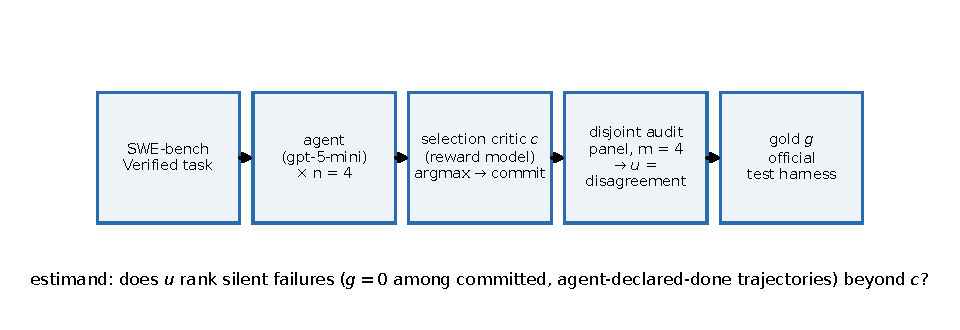
\includegraphics[width=\linewidth,height=5.0in,keepaspectratio]{figures/fig_design.pdf}\end{center}
\end{tcolorbox}
\begin{tcolorbox}[poster,colback=pale,colframe=ink,title=Takeaway for anyone building review layers for AI output,colbacktitle=ink]
Evaluate an auditor on the outputs that ship, against the score you already have, with executed ground truth. Agreement among models is not a check; each model's own judgment is worth something, their disagreement is not. The thing that caught every failure here was running the real tests.
\end{tcolorbox}
\end{minipage}\hfill
\begin{minipage}[t]{0.335\textwidth}\vspace{0pt}
\begin{tcolorbox}[poster,title=Result: a bound{,} not an absence]
Disagreement alone ranks failures at \textbf{0.508} and \textbf{0.565} AUROC. Added to the selector's own score, the gain is indistinguishable from zero on every estimator:

\begin{center}\renewcommand{\arraystretch}{1.25}
\begin{tabular}{llrr}\toprule
Population & Estimator & $\Delta$AUROC & 95\% CI \\\midrule
Verified (34 rows, 12 failures) & registered LORO & $-0.114$ & $[-0.37, +0.22]$ \\
Multilingual (77, 35) & registered LORO & $+0.005$ & $[-0.19, +0.22]$ \\
Pooled (111, 47) & logistic LORO & $-0.030$ & $[-0.10, +0.04]$ \\
Pooled & 5-fold, clustered & $-0.014$ & $[-0.09, +0.07]$ \\
Pooled & fixed unit weights & $+0.013$ & $[-0.07, +0.12]$ \\\bottomrule
\end{tabular}\\[4pt]{\fontsize{24}{29}\selectfont\color{mute} The per-benchmark LORO rows are the registered endpoint. Pooling across benchmarks was added after registration and is descriptive.}\end{center}

\begin{center}\bignum{$+0.12$}\\[4pt]{\fontsize{33}{39}\selectfont loosest pooled upper bound on what disagreement adds,\\ over 47 failures and 46 repositories. The bar we declared actionable in advance was $+0.05$.}\end{center}

With 47 positives this is a \textbf{failure to detect gain}, not evidence of absence; equivalence would need roughly five times the failures. It held across 4k--16k contexts, pruned windows, eight reward models from 1B to 32B, two re-selection regimes and a panel of LLM judges.
\end{tcolorbox}

\begin{tcolorbox}[poster,title=The pilot's positives did not travel]
\begin{center}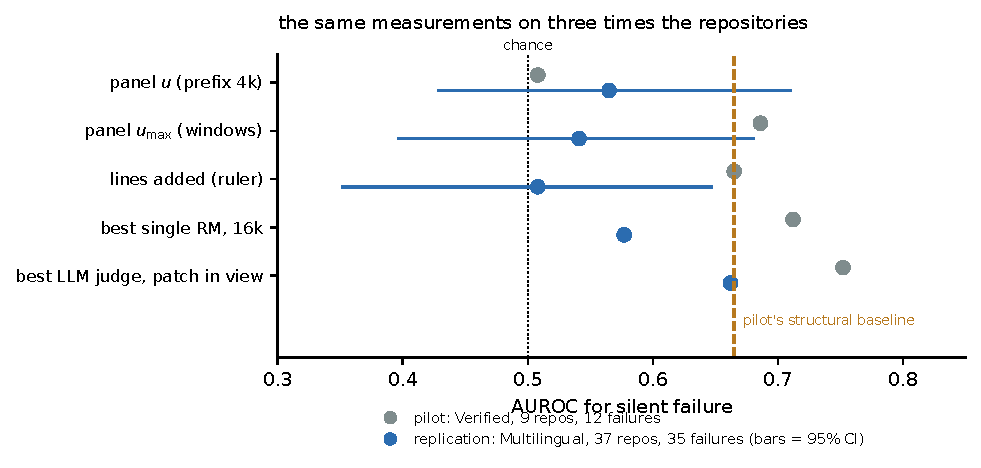
\includegraphics[width=\linewidth,height=6.8in,keepaspectratio]{figures/fig_replication.pdf}\end{center}
On 37 fresh repositories, $u_{\max}$ fell from 0.686 to 0.541 and the 1B critic from 0.712 to 0.485. Every pilot configuration that crossed a bar did so on 12 positives, and none survived the replication.
\end{tcolorbox}
\end{minipage}\hfill
\begin{minipage}[t]{0.315\textwidth}\vspace{0pt}
\begin{tcolorbox}[poster,title=Why the population matters]
\begin{center}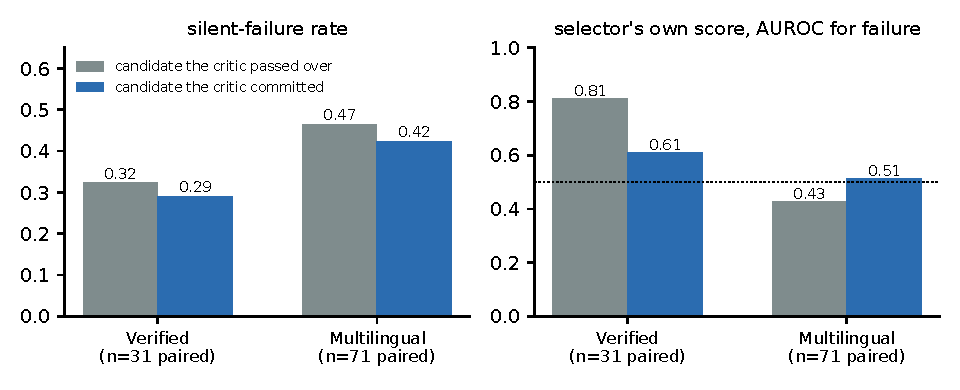
\includegraphics[width=\linewidth,height=5.8in,keepaspectratio]{figures/fig_control.pdf}\end{center}
On Verified the selector's own score ranks failures at \textbf{0.81} among candidates it passed over and \textbf{0.61} among the ones it committed, on the same instances. Pool performance does not answer the deployment question.
\end{tcolorbox}

\begin{tcolorbox}[poster,title=The critics are fine. Disagreement is the wrong statistic.]
\texttt{gpt-6-sol} ranks silent failures at \textbf{0.776} on the replication and \textbf{0.826} on the pilot; the disagreement of that newer pair falls to \textbf{0.41}. Test--retest shows the critics are stable ($r\geq0.98$): the failure is in what disagreement measures, not in critic noise.

\textbf{Post hoc, at reviewers' request:} add \texttt{gpt-6-sol}'s \emph{own} score to the selector under the same protocol and the gain is \textbf{$+0.18$ [$+0.10$, $+0.28$]} on Multilingual, $+0.14$ [$-0.02$, $+0.28$] on Verified, $+0.17$ [$+0.10$, $+0.25$] pooled (fixed unit weights, LORO). Not pre-registered. The critic's judgment carries; its disagreement with others does not.
\end{tcolorbox}

\begin{tcolorbox}[poster,title=Seven ways the instrument lied to us]
Each would have produced a publishable result: a sandbox flag that hid \texttt{numpy} from the gold harness; a judge emitting three values over 640 candidates; image pulls failing (41/41 ``failures'' in 499 s); a power function reporting 0.40 under the null; repository grouping that truncated hyphenated names; rank normalisation fit on all rows; a selector-axis filter that manufactured $+0.375$ where the correct population gives $+0.012$.

\textbf{Rule adopted:} a rate of exactly 0\% or 100\%, or a statistic that cannot move, is an instrument reading, not a result.
\end{tcolorbox}

\begin{tcolorbox}[poster,title=A stronger agent,colbacktitle=ink]
Amendment 13: \texttt{DeepSeek-V4.1-Flash}, 114 Multilingual instances, 100 steps. Failure rate \textbf{0.200} over 456 attempts (four per instance) vs \textbf{0.579} for \texttt{gpt-5-mini} over 114 (one per instance) at the same 100-step cap; the capability gate passed, but \textbf{no critic cleared the 0.65 selector bar} (gpt-5 judge 0.552; reward models 0.419--0.523; gpt-6-sol 0.619), so the cell is descriptive only.
\end{tcolorbox}
\end{minipage}


\end{document}
